%!TEX root = ../report.tex
\documentclass[a4paper,12pt,twoside,openany]{memoir}

\usepackage[english]{babel}

\usepackage[utf8]{inputenc}

\usepackage[T1]{fontenc}

\usepackage{graphicx}

\usepackage{color}
\usepackage{xcolor}

\usepackage{moreverb}
\usepackage{fancyvrb}
\usepackage{listings}
\usepackage{caption}
\usepackage{courier}
\usepackage{float}
\usepackage{amsmath}
\usepackage{amssymb}

\usepackage{hyperref}
\usepackage{natbib}

\usepackage{wrapfig}

\usepackage{pdflscape}

\usepackage{lscape}

\usepackage{rotating}

\usepackage{lastpage}
\let\footruleskip\undefined
\usepackage{fancyhdr}

% Awesome todo notes
\usepackage[colorinlistoftodos]{todonotes}
\setlength{\marginparwidth}{2cm}
\reversemarginpar

% Cool chapter headings
\usepackage{tikz}
\usepackage{kpfonts}
\usepackage[explicit]{titlesec}
\newcommand*\chapterlabel{}
\titleformat{\chapter}
  {\gdef\chapterlabel{}
   \normalfont\sffamily\Huge\bfseries\scshape}
  {\gdef\chapterlabel{\thechapter\ }}{0pt}
  {\begin{tikzpicture}[remember picture,overlay]
    \node[yshift=-3cm] at (current page.north west)
      {\begin{tikzpicture}[remember picture, overlay]
        \draw[fill=lightgray] (0,0) rectangle
          (\paperwidth,3cm);
        \node[anchor=east,xshift=.9\paperwidth,rectangle,
              rounded corners=20pt,inner sep=11pt,
              fill=darkgray]
              {\color{white}\chapterlabel#1};
       \end{tikzpicture}
      };
   \end{tikzpicture}
  }
\titlespacing*{\chapter}{0pt}{50pt}{-60pt}

% Code
\lstset {
    basicstyle=\footnotesize\ttfamily,
    numbers=left,
    numberstyle=\tiny,
    stepnumber=1,
    numbersep=5pt,
    tabsize=2,
    language=C,
    extendedchars=true,
    breaklines=true,
    keywordstyle=\color{black}\bfseries,
    frame=b,
    stringstyle=\color{gray}\ttfamily,
    showspaces=false,
    showtabs=false,
    xleftmargin=17pt,
    framexleftmargin=17pt,
    framexrightmargin=5pt,
    framexbottommargin=4pt,
    showstringspaces=false
}
\DeclareCaptionFont{white}{\color{white}}
\DeclareCaptionFormat{listing}{\colorbox[cmyk]{0.43, 0.35, 0.35,0.01}{\parbox{\textwidth}{\hspace{15pt}#1#2#3}}}
\captionsetup[lstlisting]{format=listing,labelfont=white,textfont=white, singlelinecheck=false, margin=0pt, font={bf,footnotesize}}
\renewcommand{\lstlistingname}{Code}

% C# language
\lstdefinelanguage{CSharp}
{
 morecomment = [l]{//}, 
 morecomment = [l]{///},
 morecomment = [s]{/*}{*/},
 morestring=[b]", 
 sensitive = true,
 morekeywords = {abstract,  event,  new,  struct,
   as,  explicit,  null,  switch,
   base,  extern,  object,  this,
   bool,  false,  operator,  throw,
   break,  finally,  out,  true,
   byte,  fixed,  override,  try,
   case,  float,  params,  typeof,
   catch,  for,  private,  uint,
   char,  foreach,  protected,  ulong,
   checked,  goto,  public,  unchecked,
   class,  if,  readonly,  unsafe,
   const,  implicit,  ref,  ushort,
   continue,  in,  return,  using,
   decimal,  int,  sbyte,  virtual,
   default,  interface,  sealed,  volatile,
   delegate,  internal,  short,  void,
   do,  is,  sizeof,  while,
   double,  lock,  stackalloc,   
   else,  long,  static,   
   enum,  namespace,  string}
}

% Pretty section headings
\usepackage{titlesec}
\titleformat{\section}{\Large\bfseries}{\thesection \hspace{0.5em} #1}{1em}{\hrule\vspace{-1em}}

\newcommand{\pdf}{PDF}

\newcommand{\Z}{\ensuremath{\mathbb{Z}}\xspace}

% Kommando, der sikrer ensartede referencer til figurer

\newcommand{\figref}[1]{Figure \ref{#1}}

\newcommand{\mgd}[2]{\ensuremath{\{ #1 \mid #2 \}}}

%\newtheorem{saetning}{S�tning}
\newtheorem{definition}{Definition}


%\def\mypart#1#2{%
%  \par\break % Page break
%  \vskip .3\vsize % Vertical shift
%  \refstepcounter{part}% Next part
%  {\centering\Large Part \thepart.\par}% 
%  \vskip .1\vsize % Vertical shift 
%  % Some text
%  #2
%  \vfill\break % Fill the end of page and page break
%}

\renewcommand{\afterpartskip}{\vfil} % The part will now not clear page
\def\mypart#1#2{% \mypart{title}{description}
\cleardoublepage
\part{#1}% Create part with 'title'
\vspace{-8cm}% Vertical shift
\begin{center}%
\begin{tabular}{p{12cm}}% Use tabular to create bigger 'margins'
\noindent #2% description
\end{tabular}%
\end{center}%
\cleardoublepage% clear page after part
}

\setlrmarginsandblock{2.5cm}{2.5cm}{*}
\setulmarginsandblock{2.5cm}{2.5cm}{*}

\checkandfixthelayout

\raggedbottom
\begin{document}

% Laver forsiden ud fra de indstillinger der er sat i preamblen.
%%  A simple AAU report template.
%  2012-04-20 v. 0.2.0
%  Copyright 2010-2012 by Jesper Kj�r Nielsen <jkn@es.aau.dk>
%
%  This is free software: you can redistribute it and/or modify
%  it under the terms of the GNU General Public License as published by
%  the Free Software Foundation, either version 3 of the License, or
%  (at your option) any later version.
%
%  This is distributed in the hope that it will be useful,
%  but WITHOUT ANY WARRANTY; without even the implied warranty of
%  MERCHANTABILITY or FITNESS FOR A PARTICULAR PURPOSE.  See the
%  GNU General Public License for more details.
%
%  You can find the GNU General Public License at <http://www.gnu.org/licenses/>.
%
%\pdfbookmark[0]{Front page}{label:frontpage}%
%\begin{titlepage}
	%\addtolength{\hoffset}{0.5\evensidemargin-0.5\oddsidemargin} % set equal margins on the frontpage - remove this line if you want default margins
	\thispagestyle{empty}
	\ThisTileWallPaper{\paperwidth}{\paperheight}{billeder/aau_cover.png}

	\vspace*{\fill}

	\noindent \colorbox{aaublue}{
		\parbox{\textwidth}{%
			\color{white}%
			\begin{center}
				\Huge{{\fontfamily{ua1}\selectfont Gift Coordination}} % insert your title here
			\end{center}
			\begin{center}
			\Large{\textsf{Group SW310e12}} % insert your subtitle here
			\end{center}
		}}

	\vfill

	\noindent \colorbox{white}{
		\begin{minipage}[b]{6.5cm}
		\begin{center}
			
\includegraphics[width=150px]{billeder/aau_new_logo}
			\end{center}
			\vspace*{-20px}
			%{\small \textcolor{aaublue}{Department of Computer Science}}  \\
			%{\small \textcolor{aaublue}{Software Engineering}}
		\end{minipage}
	} 
	\hfill  
	\colorbox{white}{ 
		\begin{minipage}[b]{3.5cm}	 
			\flushright
			{\large Autumn 2012} \\
			%{\small Group SW310e12}\\
		\end{minipage}
	}

%\end{titlepage}
\clearpage

\section{Reading guide}
Hi Radu, we are now ready for you to make the final corrections for the following part:

Introduction (part 1), and Arduino (part 2).

We haven't changed much in the rest of the report because we are working on the coding. % Reading guide for the supervisor
\cleardoublepage

\frontmatter
%% Dette er LaTeX-versionen af titelbladet for tek-nat-basis-rapporter 2004 efter?r
% Filen kr?ver:
% Universitetets logo:  aau-logo.png (for LaTeX) eller aau-logo.ps (for LaTeX)
% Synopsis: En fil ved navn synopsis.tex

% Udarbejdet af: Hans H?ttel (hans@cs.auc.dk) 21. maj 2003
% Rettet af Morten Christophersen (mortench@tnb.aau.dk) 30. nov 2004(?ndret til nyt design 2004 efter?r)

%\documentclass[11pt]{article}
%\ifx\pdfoutput\undefined 
%\usepackage[dvips]{graphicx}
%\else
%\usepackage[pdftex]{graphicx} 
%\usepackage{type1cm} \fi
%    \usepackage[ansinew]{inputenc}
%    \usepackage{a4}

%\begin{document} 
\thispagestyle{empty}
%\begin{titlepage}
\begin{nopagebreak}
{\samepage 

\begin{tabular}{r}
\parbox{\textwidth}{  \raisebox{-10mm}{
\includegraphics[width=120px]{billeder/aau_new_logo}}
\hfill \hspace{2cm} \parbox{8cm}{\begin{tabular}{l} %4.90
{\small \textbf{\textcolor{aaublue}{\fontfamily{cmr}\selectfont 3rd Semester - Software Engineering}}}\\
{\small \textbf{\textcolor{aaublue}{\fontfamily{cmr}\selectfont Department of Computer Science}}}\\ 
{\small \textcolor{aaublue}{{\fontfamily{cmr}\selectfont Selma Lagerløfs Vej 300}}} \\
{\small \textcolor{aaublue}{{\fontfamily{cmr}\selectfont 9220 Aalborg ?}}} \\
\end{tabular}}}
\end{tabular}

\begin{tabular}{cc}
\parbox{7cm}{
\begin{description}

\item { Title:} 

Gift Coordination\\
  
\item { Theme:} 

From users to data, algorithms and tests - and back again

\end{description}

\parbox{8cm}{

\begin{description}
\item { Project period:}\\
   P3, fall semester 2012\\
   September 3rd 2012 \\
   to December 20th 2012
  \hspace{4cm}
\item { Project group:}\\
  SW411F13
  \hspace{4cm}
\item { Participants:}\\
Andreas Abildgaard \\
Jonas Steen Hansen \\
Mathias Nielsen \\
Michel Laden \\
Morten Fjelsted Baagøe \\
Morten Møller Jacobsen \\
\hspace{2cm}
\item { Supervisor:}\\
Radu Mardare
  
\end{description}
}
\begin{description}
\item { Prints: 9 }
\item { Pages: 84 } 
\item { Appendices: 1} 
\item { Concluded 20/12-2012} 
\end{description}
\vfill } &
\parbox{7cm}{
  \vspace{.15cm}
  \hfill 
  \begin{tabular}{l}
  { Abstract}\bigskip \\
  \fbox{
    \parbox{6.5cm}{\bigskip
     {\vfill{\small This report documents the problem of creating a simplified version of Arduino language along with a compiler to translate from this simplified version to Arduino. The report describes the process of completing this task and takes into account how the product holds up against Arduino language. Both pre analysis, actual implementation and testing of the invented language are described in detail. The report furthermore includes the theory needed to understand the steps taken. At the end of the report the product is evaluated and the choices reflected upon.
     \bigskip}}
     }}
   \end{tabular}}
\end{tabular}} \vspace{1.3cm}
\\ \\ 
\end{nopagebreak}
%\end{titlepage}
%\end{document}

\cleardoublepage

% De vigtigste forskelle mellem \include og \input ligger i at
% \include kun m? findes EFTER preamblen og at 
% inkluderede filer kan frav?lges ved generering af output
% ved brug sammen med \includeonly.

% Se arbejdsblad-skabelon.tex for et eksempel herp?.

%\include{formalia/forord}

% For at sikre sideskift efter forord. Denne kommando b?r kun bruges i
% absolutte undtagelsestilf?lde.

%\newpage
%\section*{Preface}

\phantom{Luft}\vspace{5cm}
\begin{table}[H]
	\centering
		\begin{tabular}{c c c}
			\underline{\phantom{JAERJAERJAERJAERGO}} & \phantom{cookies} & \underline{\phantom{JAERJAERJAERJAERGO}} \\
			Andreas Abildgaard			& \phantom{cookies} & Jonas Steen Hansen		\\
			&&\\
			&&\\
	   		\underline{\phantom{JAERJAERJAERJAERGO}} & \phantom{cookies} & \underline{\phantom{JAERJAERJAERJAERGO}} \\
			Mathias Nielsen 					& \phantom{cookies} & Michel Laden 			\\			
			&&\\
			&&\\
	   		\underline{\phantom{JAERJAERJAERJAERGO}} & \phantom{cookies} & \underline{\phantom{JAERJAERJAERJAERGO}} \\
			Morten Fjeldsted Baagøe 					& \phantom{cookies} & Morten Møller Jacobsen 			\\			
			&&\\
			&&\\			
		\end{tabular}
\end{table}

\pagebreak

\tableofcontents*
\mainmatter

%Main parts of report
\part{Introduction}\pagebreak
\chapter{Introduction}
\section{Introduction}
When programming for the first time, most code can seem unintuitive and can be hard to understand. A beginner can make crucial mistakes and have a hard time learning how to program without having a teacher instructing them.\\

Programming languages differ in various aspects and some are more intuitive for beginners than others. Some languages are complex which often is due to the fact that they have a lot of features. For a beginner, the complexity of having several different methods to produce the same outcome, is obsolete and can make a language difficult to learn. \\

When programming for the first time, a programmer can choose to start with any language. A beginner with interest in learning about smaller hardware is likely to encounter the programming language of Arduino. Arduino gives programmers the option to program components and use them for a wide variety of purposes. Since Arduino is a small board with just one processor for input and output, the options are relatively few, and it is easy to get an overview. However the programmer can also attach other boards to the Arduino, which will add to the complexity of what the programmers has to understand in order to achieve the desired outcome. \\

The Arduino language is based on C and C++, which are languages that can be seen as cryptic and unintuitive to programmers. C for example has no boolean type, which means that the programmer has no option to check for true/false. /todo{Ved vi det med sikkerhed? At der ikke findes bool ydtryk i C} It has to be created first. C can also seem unintuitive for a beginner. For example when creating an array to hold 3 characters, the array has to be of size 4.  Without prior experiences with programming, C and C++ can be hard languages to learn. \\

With the Arduino being a good place to start for a beginner, it is not optimal that the programming language is not on par. \todo{Lidt tynd begrundelse om hvorfor Arduinos sprog ikke er begyndervenligt} Therefore this project will look into giving beginners an alternative to the Arduino language by creating a new language and a compiler for it. This language will attempt to achieve userfriendliness for beginners. A place to draw inspiration from is Python, which is a programming language praised for being intuitive and easy to learn. \todo{Kilde?} Python is declarative which means that code can be read logically. \todo{Kilde?} Thus the programmer might think that the code can look somewhat like the English language. It is easy to understand because what you write is what you get, it is not cryptic in any way. It is this kind of user friendliness that will be sought in this project.
\section{Motivation}\label{introduction:motivation}
The Arduino language is based on C and C++, which are languages that can be seen as cryptic and unintuitive to newly started programmers. An example of C not being intuitive is when creating an array to hold 3 elements, and the array has to be set to a size that can hold 4 elements. This is needed because there is a special sign to mark the end of an array (zerobit), which takes a slot itself. The programmer can work around it and/or create the functionality, but to the inexperienced programmer it adds complexity. Without prior experience with programming, C and C++ can be difficult languages to learn. \\
For beginners it could be better if the Arduino language, was simpler and easier to understand. The Arduino language is built upon C and C++, and therefore has similar flaws, at least from a beginners perspective. This project will look into giving beginners an alternative to the Arduino language by creating a new language along with a translator. A translator is needed in order to be recognizable as proper code for Arduino. This language will attempt to achieve user-friendliness with beginners in mind. A place to draw inspiration from is Python, which is a programming language praised by many experienced and inexperienced programmers for being intuitive and easy to learn. \cite{python:about} Python is a declarative language, which means that the code can be read logically. The programmer will discover that Python looks somewhat like English language. It is easier to understand because the code can be less cryptic compared to other languages. It is this kind of user friendliness that will be sought in this project.
\section{Compiler}
If a programmer should be able to avoid using Wiring when coding for the Arduino it requires two things. First of all it obviously requires another language in which the programmer can write the desired code. For this code to function on the Arduino a translator is however also required. This makes the creation of a new language a two step progress, as it is not enough to design a language. Without very well-defined translations into another known language, the invented language literally has no meaning. Therefore a translator has to be created alongside with the language. This is called a compiler and can actually be quite complex. This is described in depth in chapter \ref{the_compiler}. The goal for this compiler is to be able to translate any code in the invented language into Wiring.
\chapter{Arduino}\label{analysis:arduino}
Arduino was created by the Interaction Design Institute Ivrea (Italy), by Massimo Banzi and David Cuartielles. They were looking for an easy and cheap way for students, who study design, to integrate micro controllers into their projects\cite{arduino:hist}. Both the board and the programming language was based on the works of Hernando Barragán, one of Massimo Banzi master thesis students \cite{Wiring:thesis}.

In this project Arduino board is used to execute the code, and show a type of output. The output will be in the form of a LCD Display. 

\section{The Hardware Components}
Arduino is a single-board micro-controller, see figure \ref{fig:Arduino_uno}.
A board consists of open source hardware, which is designed around an 8-bit Atmel AVR micro-controller. Arduino boards varies in sizes. Arduino Uno board for example, has a max width of 2.1'' (5,33cm) and a length of 2.7'' (6,86cm).  \\

\par
\raisebox{-.5\height}{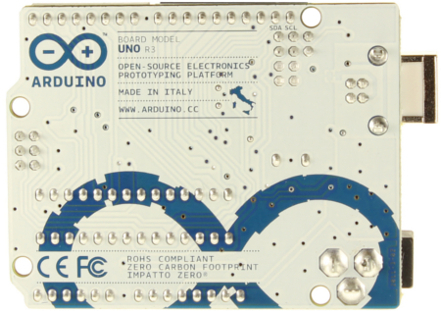
\includegraphics[width=6.5cm]{billeder/ArduinoUno_R3_Back_450px.jpg}}
\hfill
\raisebox{-.5\height}{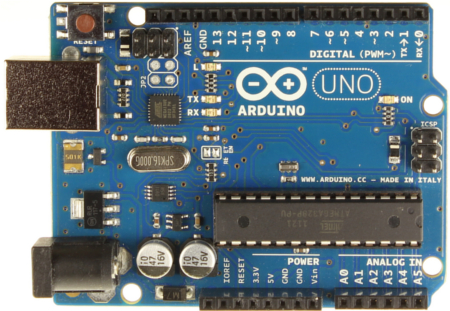
\includegraphics[width=6.5cm]{billeder/ArduinoUno_R3_Front_450px.jpg}}
\begin{figure}[H]
\caption{Picture of back- and fronside of the Arduino Uno board \cite{Arduino:board_pics}}
\label{fig:Arduino_uno}
\end{figure}
\par

\par
\raisebox{-.5\height}{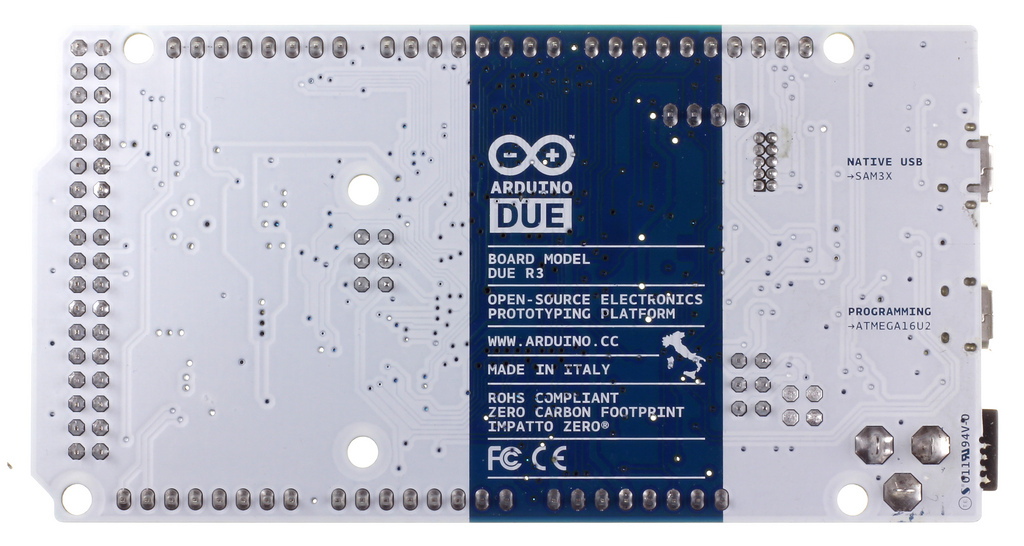
\includegraphics[width=6.5cm]{billeder/ArduinoDue_2.jpg}}
\hfill
\raisebox{-.5\height}{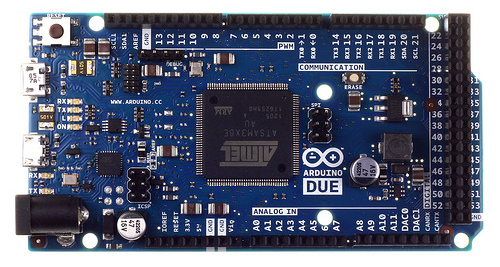
\includegraphics[width=6.5cm]{billeder/ArduinoDue_1.jpg}}
\begin{figure}[H]
\caption{Picture of back- and fronside of the Arduino Duo board \cite{Arduino:board_pics}}
\label{fig:Arduino_duo}
\end{figure}
\par

\subsection*{Specifications}
The board provides some input and output possibilities. The Arduino Uno, figure \ref{fig:Arduino_uno}, has 14 digital I/O and 6 analog inputs, where as the Arduino Due, figure \ref{fig:Arduino_duo}, has 54 digital, and 12 analog pins. The I/O functions are placed on top of the board, and are freely accessible, and consist of 0.1'' female headers. Besides the I/O there is also a Power connector, which almost in all cases require 5 volt DC. There is an USB connection on the board, so that processing data to the micro-controller is possible, though it is shown as a virtual com-port on the connected computer. However, on older boards, instead of the USB connection, a RS232 were used for serial communication. 

\begin{figure}[H]
\centering
\begin{tabular}{|c|c|}
\hline 
Microcontroller & ATmega328 \\ 
\hline 
Operating Voltage & 5V \\ 
\hline 
Input Voltage (recommended)	 & 7-12V \\ 
\hline 
Input Voltage (limits) & 6-20V \\ 
\hline 
Digital I/O Pins & 14 (of which 6 provide PWM output) \\ 
\hline 
Analog Input Pins & 6 \\ 
\hline 
DC Current per I/O Pin & 40 mA \\ 
\hline 
DC Current for 3.3V Pin & 50 mA \\ 
\hline 
Flash Memory & 32 KB (ATmega328) of which 0.5 KB used by bootloader \\ 
\hline 
SRAM & 2 KB (ATmega328) \\ 
\hline 
EEPROM & 1 KB (ATmega328) \\ 
\hline 
Clock Speed & 16 MHz \\ 
\hline 
\end{tabular} 
\caption{Hardware specifications for the Arduino Uno}
\end{figure}

On the board there is a LED, which is connected to the digital pin 13. When this diode is set to ``HIGH'' it will be turned on, and if its value is ``LOW'' it turns off. Besides the LED, there is also a reset button. If the button is pressed the micro-controller is reset. 

The specifications, which are important to take into consideration in regard to designing a programming language aimed at the Arduino platform, is the flash memory, the main memory(SRAM) and the CPU speed. The most limiting factor to take into consideration is the amount of RAM, the larger and more complex the data structures are, the bigger the risk of running out of memory while executing a program. Although this is not limited to developing for the Arduino platform, it is certainly a larger factor, then when developing for desktop computers.
Another factor that need attention is the flash memory, meaning the pace available for the program, the smallest example code for the Arduino, the Blink example listings \ref{lst:blink}, only uses 1084 bytes, which is approximately $3.3 \%$ of the total memory available. 

\begin{table}[h!]\scriptsize
\centering
\begin{tabular}{cc} 
\begin{minipage}{6cm}
{\begin{lstlisting}[caption=Arduino,frame=none,resetmargins=true,label={lst:blink}]
int led = 13;
void setup() {                
  pinMode(led, OUTPUT);     
}

void loop() {
  digitalWrite(led, HIGH);   
  delay(1000);    
  digitalWrite(led, LOW);  
  delay(1000);
}
\end{lstlisting}}
\end{minipage}
  & 
\begin{minipage}{10cm}
{\begin{lstlisting}[caption=C\#,frame=none,resetmargins=true,label={lst:C_hello}]
namespace hello
{
  class Program
  {
    static void Main(string[] args)
    {
       System.Console.WriteLine("Hello, World!");
       System.Console.ReadKey();
    }
  }
}
\end{lstlisting}}
  \end{minipage}
 \\ 
 \end{tabular} 
 \caption{Comparison between a simple Arduino and C\# example}
 \end{table} 

If a language has a lot of complex features, it will quickly run out of space. For instance with more complex languages like C\#, a simple hello world, listings \ref{lst:C_hello}, program uses 5120 bytes, and they can quickly run in the hundreds or thousands of kilobytes. This is even more important to remember, when one takes into account, that there are many different Arduino configurations, and the language have to function on all of them. The Arduino Nano for instance, only has 16 KB of memory, and there are Arduino clones by other manufactures with even less.



\subsection*{Components}
What makes Arduino such a good platform for beginners to learn to program on, is because it is really easy to connect a wide variety of components to it, making it possible for the Arduino to interact with the real world.

\begin{itemize}
\item[] \textbf{LED's} come in all size, shapes and colors, ranging from small pin size single color LED's, to large multi color LED displays.
\begin{figure}[H]
\centering
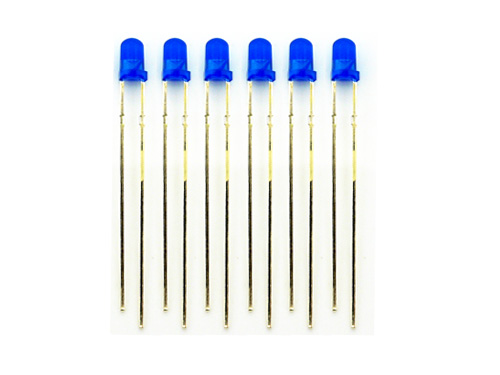
\includegraphics[width=5cm]{billeder/led.jpg}
\caption{3mm blue led}
\end{figure}
\item[] \textbf{Sensors} are some of the main components behind the Arduino success. They give the Arduino the ability to sense its surroundings. For instance the temperature of the room, whether the light is on of off, even advanced sensors like humidity, or gas sensor.
\begin{figure}[H]
\centering
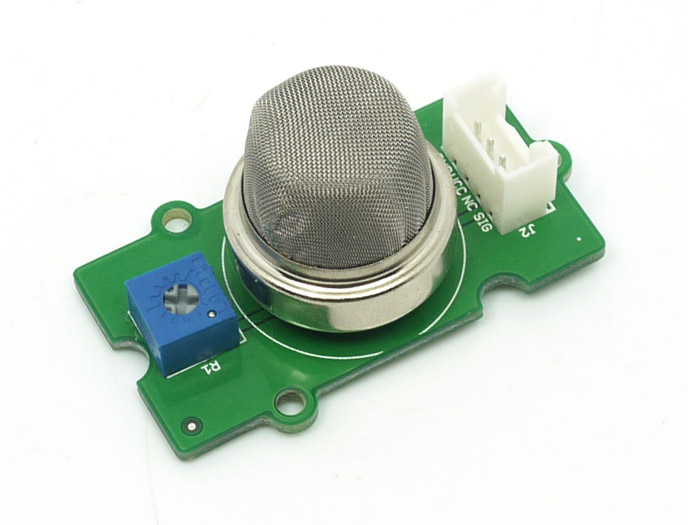
\includegraphics[width=5cm]{billeder/Sensor.jpg}
\caption{Gas sensor}
\end{figure}
\item[] \textbf{Motors} gives Arduino the ability to manipulate its surrounding, and act on the informations obtained from the sensors. There are two kind of motors, normal motors which can just be turned on/off. They are great for powering wheels or tracks. There are stepper motors, with these it is possible to control the exact amount of rotation. A more advanced version of the stepper motors are servo motors, with which more precise control is possible.
\begin{figure}[H]
\centering
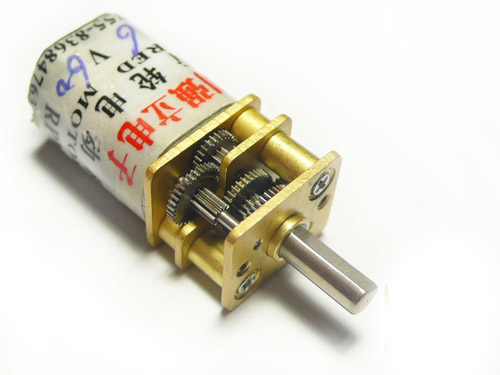
\includegraphics[width=5cm]{billeder/Motor.jpg}
\caption{Geared stepper motor}
\end{figure}
\item[] \textbf{Displays} are available in a wide range. Ranging from simple 2 line mono color LCD displays, all the way up to large OLED color and touch displays. 
\begin{figure}[H]
\centering
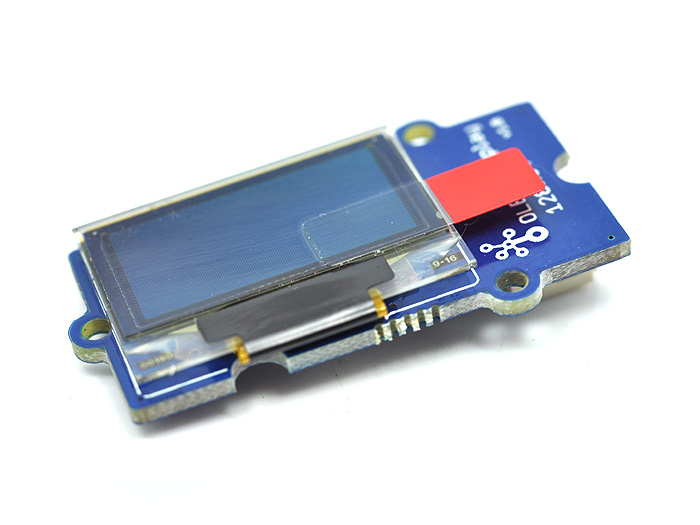
\includegraphics[width=5cm]{billeder/display.jpg}
\caption{OLED touch display}
\end{figure}
\item[] \textbf{Communication} components are easy to connect up on Arduino. This is allows it to communicate with other devices through either RF signals, Bluetooth, WiFi, cellular or just Ethernet connection.
\begin{figure}[H]
\centering
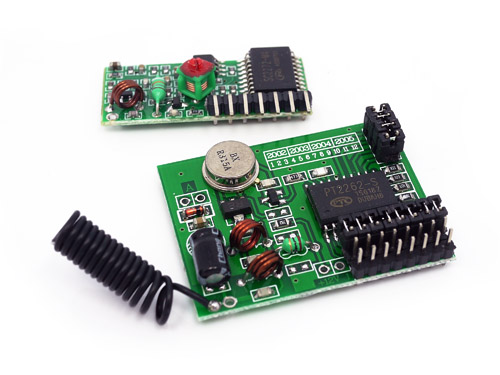
\includegraphics[width=5cm]{billeder/com.jpg}
\caption{RF transmitter and reciever}
\end{figure}
\item[] \textbf{Shields} are the components that makes the Arduino Platform great. They offer great  to the platform by allowing them to be plugged directly on to the Arduino. This makes it possible for anyone without any experience in electronics  to use them Shields are boards much like Arduino itself, but they offer all the capabilities of the components mentioned above.
\begin{figure}[H]
\centering
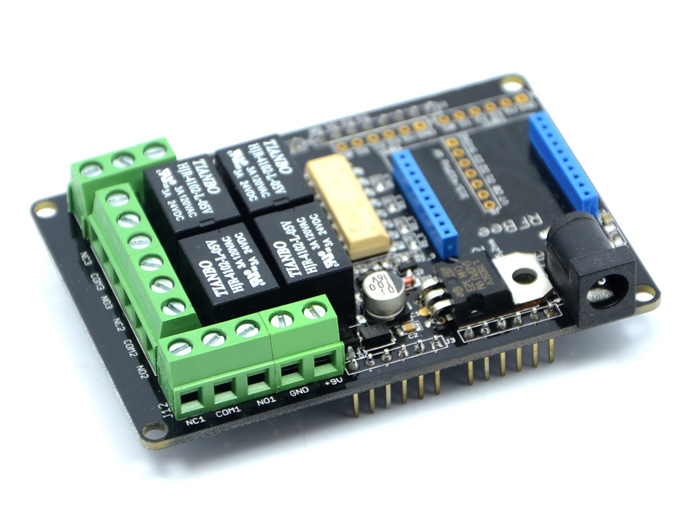
\includegraphics[width=5cm]{billeder/Shield.jpg}
\caption{Relay shield}
\end{figure}

\end{itemize}



\chapter{Analysis}

\part{Implementation}
\chapter{JavaCC - Java Compiler Compiler}
JavaCC is a parser generator that generates a fully functioning parser. JavaCC takes a file containing EBNF grammar and then makes a program that can recognize matches between the input code and the grammar, this part of the parser is called the scanner. JavaCC also creates other things like e.g. an AST (Abstract Syntax Tree, page \todo{Jonas: add section about AST in the compiler chapter, and add reference here.}) that decides the derivation of the code. \cite{JavaCC}

The process of a parser program:
\begin{itemize}
\item Input a set of token definitions, grammar and actions
\item Outputs a Java program which performs lexical analysis
	\begin{itemize}
	\item Finding tokens.
	\item Parses the tokens according to the grammar.
	\item Executes actions.
	\end{itemize}
\end{itemize}


\section{Grammar example}
Code table \ref{lst:javacc-grammar-example} is containing an example of how a grammar for an ``if''-statement can be constructed. The grammar in the example states the following:

\begin{itemize}
	\item Skip all whitespace and newlines.
	\item An ``if''-statement consists of a condition (C), a statement (S)  and optionally an ``else statement'' which contains a Statement (S)·
	\item A condition (C) consists of the string ``TBD'' - not anything else.
	\item A statement (S) also consists of the string ``TBD'' or a new ``if''-statement
\end{itemize}

\begin{lstlisting}[captionpos=b, caption={One of JavaCC's standart examples on how to make a grammar that accepts ``if''-statements.}, label=lst:javacc-grammar-example]

PARSER_BEGIN(Example)

public class Example {

  public static void main(String args[]) throws ParseException {
    Example parser = new Example(System.in);
    parser.IfStm();
  }

}

PARSER_END(Example)

SKIP :
{
  " "
| "\t"
| "\n"
| "\r"
}

void IfStm() :
{}
{
 "if" C() S() [ "else" S() ]
}

void C() :
{}
{
  "TBD"
}

void S() :
{}
{
  "TBD"
|
  IfStm()
}
\end{lstlisting}

%inputs go here

\chapter{Test}
This section will look at the testing of the different aspects of the process, and describe these how tests were done. The focus of the tests will be on lexical analysis and the compiler.

\subsection*{Testing method}
There are a wide variety of methods for testing computer software, these can be broken into two main groups, white box and black box testing. The difference between the two are, that with black box test the focus is not on what happens inside the program, but rather look at the program as a box that receives an input and returns an output based on the input. whereas with white box testing, the focus is as much on how the code is running as on the output.\\

The Advantages of the two different methods are:
\begin{itemize}
\item[] \textbf{Black box} It is not necessary to have any knowledge of the code, the tester only needs to know how to pass the input parameter. This also makes it faster to run and evaluate the tests, since the 
\item[] \textbf{White box} Since it tests the code, it is possible to use these tests to optimize the code, although this kind of testing requires a expert knowledge of the code to design the tests. 
\end{itemize}   

\begin{tabular}{|c|c|c|c|}
\hline 
Test  & Expected result & Actual result  & Passed \\ 
\hline 
void setup()do
end &
void setup()\{
\} &
void setup()\{
\} & 
\checkmark  \\ 
\hline 
• & • & • & \checkmark \\ 
\hline 
• & • & • & \checkmark \\ 
\hline 
\end{tabular} 
\part{Discussion}
\cleardoublepage
%inputs goes here
\section{Evaluation of the Product}

\section{Improvement}\label{discussion:improvements}
By comparing the finished project with the MoSCoW analysis, every feature within the category ''must have`` has been achieved with the exception of the ability to define functions. However the ability to call already existing functions is possible, which makes the programmer able to use the various Arduino libraries. Additionally, PH could be improved by adding more data types, and more functionality in form of control structures. \\

An important improvement for the compiler, is the ability to compile directly from PH to machine code, without the need of an external Arduino language compiler. This is because the task of compiling from PH to machine code would be a lot simpler.\\

The language does not currently take reserved words in the Arduino language into consideration, which should be solved because these words can result in errors when compiling the Arduino language to machine code. If the programmer declares a variable with the same name as a reserved word in the Arduino language it may create problems. \\ 
\section{Conclusion}

In this project we have attempted to create a language for Arduino as described in \ref{analysis:source-language}. The main target features are that it should be simpler and easier to use than the official language along with being intuitive, even for beginners. \\
The resulting language is stripped from duplicate methods of producing similar outcomes. For example, loops has been limited to while, and variables containing numbers has been limited to only include integers and floats. This is seen in \ref{analysis:informal-specification}. Removing redundant parts of the language has resulted in a smaller language, consequently making the new language easier to overview. Different to the official Arduino language, our language does not have the need to parenthesize elements such as if-statements or loops. Instead the language achieves more readability and intuitivity by using the keywords do and end. This approach is also used in boolean expressions where keywords such as and and or are used rather than \&\& and  ||. The similarity to the English language makes the language more intuitive to learn and use because it is more similar to a language that any English-speaking people are familiar with. As such the overall goals has been achieved to some degree. \\
The task of writing a translator which can convert a program from our language to Arduino has been achieved and the progress documented by the report. The validity of the translation is verified by the tests performed in \todo{Morten: Ref til test+conclusion on the test}. The tests show that blablabla. \\
Comparing the finished project with the MoSCoW model described in \ref{analysis:moscow}, every feature within the category of must have has been achieved with the exception of functions (Including parameters and return values). As described in the MoSCoW definition of must have, this has great impact on the language. The resulting language is impaired in that it is unable to make calls to execute statements, meaning that code can not be reused. This makes the language unsuited for any programming where this functionality is desired. \\
Of the less important features, the ability to print along with advanced operators has been implemented. We did however not get around to implement other loops than while, even though a foreach loop was desired. This does however not impair the functionality of the language and is a matter of convenience. \\
The language does not currently respect reserved words in Arduino language which is something that should be solved as using these words will result in an error when compiling from Arduino to machine code. The language does not deal with the need for parenthesization in arithmetic expressions and leaves this job to the Arduino compiler.

In conclusion, the language has achieved the base goals set for it. It does however feel unfinished, and could be developed further for considerable improvements. While the product demonstrates the philosophy of the new language well, the solution is not optimal as a programming language without improvements.\\
\todo{Morten: Mangler muligvis noget om Vikings hardware error}


%Liste over todo notes
\listoftodos



%Problemanalyse

%Matematik og algoritmer

%Programdesign

%Test

%Konklusion


\bibliographystyle{alpha}
\bibliography{litterature/litteratur}

% Appendix
\appendix

\end{document}